\subsubsection{Registro de usuario}

En el registro del usuario se deberá solicitar al usuario su nombre, correo electrónico y contraseña, que será enviada al orquestrador en texto plano para su registro, si es exitoso el orquestrador deberá enviar un mensaje de confirmación al usuario.

\begin{figure}[h!]
    \centering
    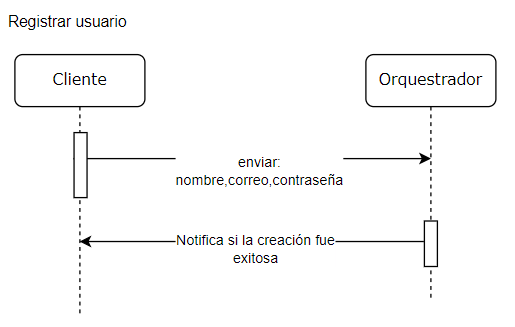
\includegraphics[width=\textwidth]{register-user.png}
    \caption{Diagrama de caso de uso: registro de usuario}
\end{figure}

\subsection{Identificación del usuario}
En esta primera version no nos preocuparemos de que la información del usuario se transmita de forma segura, por lo que el usuario deberá identificarse con un nombre de usuario, correo electrónico y contraseña. Que será enviada al orquestrador en texto plano para su verificación.

\begin{figure}[h!]
    \centering
    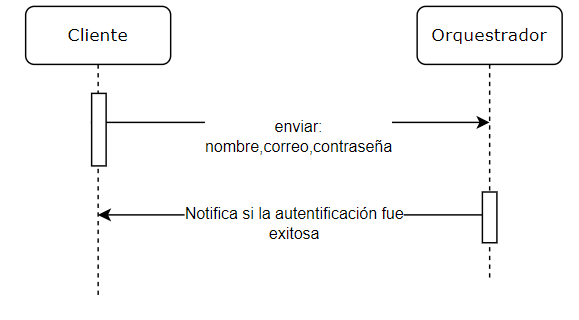
\includegraphics[width=\textwidth]{login-user.png}
    \caption{Diagrama de caso de uso: identificación del usuario}
\end{figure}


\subsection{Registro de una red privada}

Deseamos que el usuario pueda registrar las redes privadas a las que desea conectarse, para ello se deberá implementar un mecanismo de registro de redes privadas.
El cliente deberá enviar un mensaje al orquestrador con el nombre de la red privada que desea crear, si la red privada existe el orquestrador deberá notificar al cliente, si la red privada no existe, el orquestrador deberá crearla y enviar un mensaje de confirmación con la información siguiente: IP asignada, rango, mascara de la red privada creada.

\begin{figure}[h!]
    \centering
    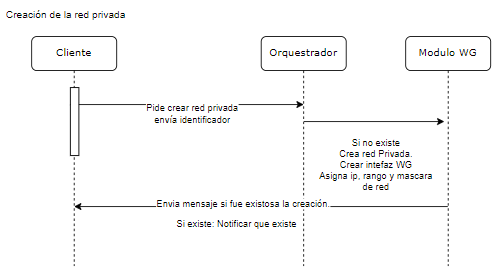
\includegraphics[width=\textwidth]{create-network.png}
    \caption{Diagrama de caso de uso: registro de red privada}
\end{figure}

Una red privada desde el punto de vista del orquestrador es un objeto que contiene la siguiente información:
\begin{itemize}
    \item Identificador
    \item Nombre de la red privada
    \item Lista de dispositivos finales
    \item Lista de conexiones
\end{itemize}

La idea es crear este objeto para almacenar y consultar datos sobre sobre las redes privadas de un cliente.
Luego el razonamiento tras crear un interfaz virtual de Wireguard es que en caso de que la comunicación entre los dispositivos finales no sea posible, el orquestrador pueda actuar como relay dentro de la red privada virtual.


\subsection{Registro de un dispositivo final}
Uno de los objetivos del orquestrador será registrar los dispositivos finales conectados a la red privada, para ello se deberá implementar un mecanismo de registro de dispositivos.

\begin{figure}[h!]
    \centering
    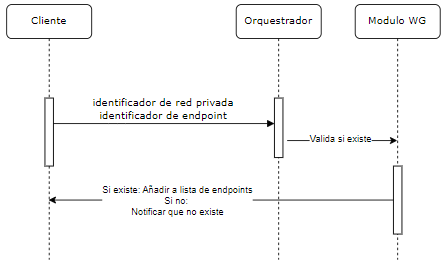
\includegraphics[width=\textwidth]{registro-endpoint.png}
    \caption{Diagrama de caso de uso: registro de dispositivo final}
\end{figure}

El cliente enviara al orquestrador el identificador de la red privada y el dispositivo final que desea registrar.
El orquestrador deberá validar que la red privada exista y que el dispositivo final no esté registrado en la red privada, si es así el orquestrador deberá registrar el dispositivo final y enviar un mensaje de confirmación al cliente.

El orquestrador sera quien asigne la IP de los dispositivos finales dentro de una red privada de los clientes. Así que tambien deberá asignar el rango y la mascara de la red privada. 

\newpage
\subsection{Cliente verifica conectividad con sus endpoint registrados}
El cliente deberá informar al orquestrador si es posible que se comunique con los demás dispositivos finales de la red privada, para ello deberá enviar un mensaje al orquestrador para conocer que dispositivos finales supone que están conectados a la red privada.
Luego este cliente verificara si alcanza a los demás dispositivos finales de la red, mediante un mensaje enviado desde la interfaz Wireguard, es decir, usando las IP asignadas por el orquestrador.

Este caso de uso se deberá hacer con cierta periodicidad, para que el cliente pueda tener información actualizada de la red privada. Y en caso de que el orquestrador la solicite el cliente tendrá la información de la red privada actualizada.

\begin{figure}[h!]
    \centering
    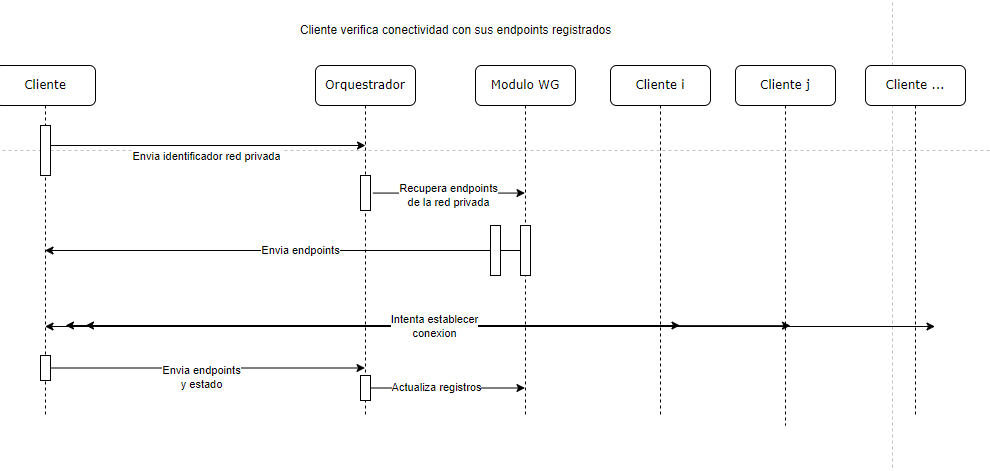
\includegraphics[width=\textwidth]{cliente-alcanza-endpoints.png}
    \caption{Diagrama de caso de uso: cliente verifica conectividad con sus endpoint registrados}
\end{figure}

\newpage
\subsection{Cliente consulta información de red privada al orquestrador}
El cliente deberá poder consultar la información de la red privada a la que está conectado, para ello deberá enviar un mensaje al orquestrador con el identificador de la red privada, el orquestrador deberá responder con la información de la red privada.

\begin{figure}[h!]
    \centering
    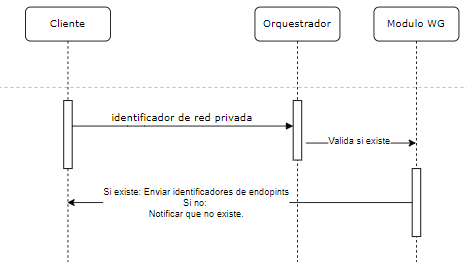
\includegraphics[width=\textwidth]{divulgar-red-privada.png}
    \caption{Diagrama de caso de uso: cliente consulta información de red privada al orquestrador}
\end{figure}


\subsection{Cliente consulta redes privadas disponibles}
El cliente deberá poder consultar las redes privadas disponibles, para ello deberá enviar un mensaje al orquestrador, el orquestrador deberá responder con la lista de redes privadas conocidas.

\begin{figure}[h!]
    \centering
    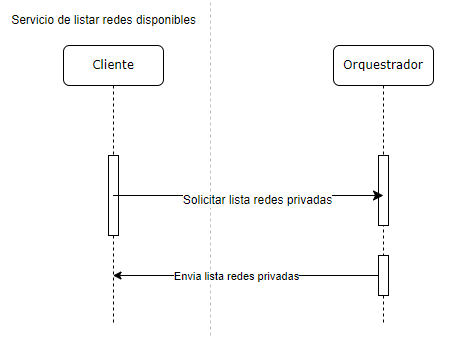
\includegraphics[width=\textwidth]{listar_redes.png}
    \caption{Diagrama de caso de uso: cliente consulta redes privadas disponibles}
\end{figure}

\subsection{Orquestrador divulga tablero de red privada}
Si el cliente envia una solicitud del estado de una red privada al orquestrador, este deberá responder con un tablero de la red privada, que contiene la información de los dispositivos finales conectados a la red privada, las conexiones entre los dispositivos finales y la alcanzabilidad de los dispositivos finales desde el punto de vista del orquestrador.

Esto se deberá hacer con cierta periodicidad, para que el cliente pueda tener información actualizada de la red privada.

\begin{figure}[h!]
    \centering
    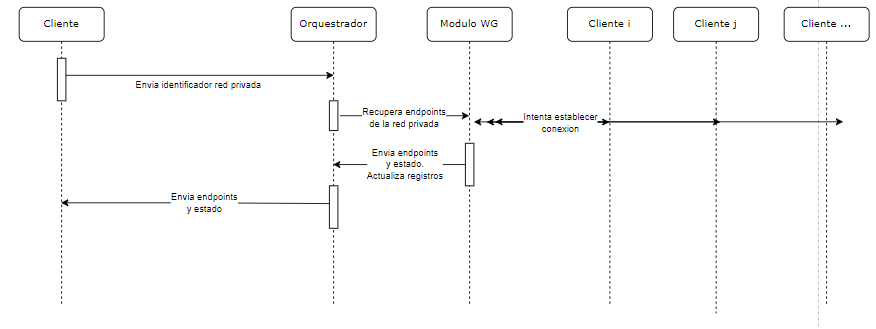
\includegraphics[width=\textwidth]{server-divulga-tablero.png}
    \caption{Diagrama de caso de uso: orquestrador divulga tablero de red privada}
\end{figure}

